%Tệp mẫu làm đề thi trắc nghiệm phiên bản 3.0
%Tác giả Nguyễn Hữu Điển (ĐHKHTN, Hà Nội)
% Đề trắc nghiệm được thiết kế trên phông Unicode,
%Đã dùng lớp examdesign.cls có sửa đổi
%Cùng với gói lệnh dethi.sty tạo ra:
%Đề thi trắc nghiệm từ một bộ đề sinh ra các câu hởi được 
%sắp xếp ngẫu nhiên và các chi tiết của câu hỏi cũng được 
%xắp sếp ngẫu nhiên. Mỗi đề thi sinh ra đều có thể in ra đáp án riêng biệt.
%examdesign.cls đòi hỏi các gói lệnh enumerate, multicol, shortlst, keyval.
\documentclass[11pt]{article}
\usepackage{amsmath,amsxtra,latexsym, amssymb, amscd}
\usepackage[utf8]{vietnam}
\usepackage{color}
\usepackage{graphicx}
\usepackage{picinpar}
\usepackage{mathptmx} 
\usepackage{enumerate}
\usepackage{multicol}
\usepackage{shortlst}

\usepackage[baithi]{dethi} %Gói lệnh cho đề thi Việt Nam
% \usepackage{fancybox}
% \cornersize*{3.6mm}
\Fullpages %Định dạng trang đề thi
\ContinuousNumbering %Đánh số liên tục các bài thi
\NumberOfVersions{1} %10 là số bài thi khác nhau được in ra
\SectionPrefix{\relax }%\bf Phần \Roman{sectionindex}. \space}
\tieudetuluan
 \tieudedapan
\chucauhoi{Câu}                %Chữ trước các số câu hỏi
\setlength{\baselineskip}{12truept}
\def\v#1{\overrightarrow{#1}} %Làm vectơ
\graphicspath{{hinh-cauhoi/}{hinh-vidu/}} %Đường dẫn của nơi để hình
 \ShortKey             %Lệnh hiện ra đáp án mỗi đề thi
\tentruong{BỘ GIÁO DỤC VÀ ĐÀO TẠO}
\tenkhoa{ĐỀ MINH HỌA}
\loaidethi{Đề gồm có 06 trang}%{ĐỀ THI LẠI}%%{ĐỀ CHÍNH THỨC}
\tenkythi{KÌ THI TRUNG HỌC PHỔ THÔNG QUỐC GIA NĂM 2017}
\tenmonhoc{Môn: Toán}
\madethi{100}
\thoigian{\underline{Thời gian làm bài: 90 phút, không kể thời gian phát đề}}
\begin{examclosing}
\centerline{-- HẾT --}
\end{examclosing}
\begin{document}
\begin{shortanswer}[title={\relax}, rearrange=no]
\begin{question}%1
Phát biểu các quy tắc tìm chu trình Hamilton. Hãy chứng minh rằng đồ thị trong hình ~\ref{fig:hinh1} có chu trình Hamilton.
\begin{figure}[!ht]
\centering
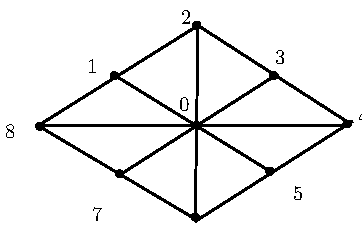
\includegraphics[scale =0.8]{hamilton}
\caption{}\label{fig:hinh1}
\end{figure}
\begin{answer}
Các quy tắc tìm chu trình Hamilton như sau:
{\it Quy tắc 1:}
Nếu đỉnh $V$ có bậc $2$, thì cả hai cạnh gắn với nó phải là một phần của chu trình Hamilton bất kì.

{\it Quy tắc 2:}
Trong quá trình xây dựng chu trình Hamilton, không có chu trình có thể tạo thành cho tới khi tất cả các đỉnh đã được ghé qua.

{\it Quy tắc 3:}
Nếu trong quá trình xây dựng chu trình Hamilton hai trong số các cạnh gắn liền với 1 đỉnh $V$ được chỉ ra, thì tất cả các cạnh gắn liền khác có thể bỏ đi được.


Xét đỉnh 0. Ta có thể chọn hai cạnh tới đỉnh này là: 

a) 01 và 05:  Xóa các cạnh tới 0 khác (theo quy tắc 3) ta còn lại đồ thị.

Các đỉnh còn lại 2, 3, 4 còn lại bậc 2. Vậy phải lấy các cạnh 12, 23, 34, 45 nhưng như vậy tạo ra chu trình con thực sự và không tạo ra chu trình Hamilton được (hình~\ref{fig:hin}).

\begin{figure}[!ht]
\begin{minipage}[b]{5cm}
\centering
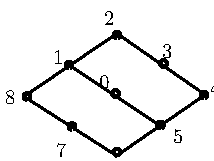
\includegraphics[scale =0.8]{hamilton1}
\caption{}\protect\label{fig:hin}
\end{minipage}
\hfill
\begin{minipage}[b]{6cm}
\centering
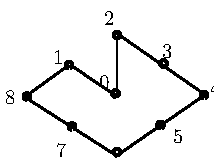
\includegraphics[scale =0.8]{hamilton2}
\caption{}\label{fig:hình3}
\end{minipage}
\end{figure}
b) 01 và 02: Xóa các cạnh tới 0 khác (theo quy tắc 3) và xóa cạnh 12 (theo quy tắc 2) ta còn lại đồ thị (hình~\ref{fig:hình3}).

Các đỉnh 3, 4, 5, 6, 7, 8 còn lại bậc hai ta nhận được chu trình Hamilton: 0234567810.

Tương tự các trường hợp chọn 01 và 03; 01 và 04 đều không được.
\end{answer}
\end{question}



\begin{question}%2
Có 10 sinh viên trong một học kì học các môn tùy chọn và các môn bắt buộc theo bảng ở hình ~\ref{fig:hinh00}. Hãy thiết lập lịch thi có ít đợt nhất   sao cho  các sinh viên này không bị nhỡ thi một môn đã học nào.
\begin{table}[!htp]
\centering
\begin{tabular}{ l  l }
 Tên sinh viên & Môn đã chọn học \\
\hline
 An & Vật lí, Toán, Tiếng Anh \\
Vân& Vật lí, Khoa học trái đất, Kinh tế\\
Lan & Khoa học trái đất, Kinh doanh\\
Hào &Thống kê, Kinh tế\\
Hùng&Toán, Kinh doanh\\
Bảo&Vật lí, Khoa học trái đất\\
Hồng& Kinh doanh, Thống kê\\
Điền &Toán, Khoa học trái đất\\
Cường&Vật lí, Môi trường, Thống kê\\
Quý&Vật lí, Kinh tế, Môi trường.
\end{tabular}
\caption{}\label{fig:hinh00}
\end{table}
\begin{answer}
Gọi các môn học là các đỉnh của đồ thị. Hai đỉnh có một cạnh nếu một trong các sinh viên đã chọn học hai môn này. Như vậy đồ thị được thiết lập như hình~\ref{fig:hinh4}. 

\begin{figure}[!ht]
\begin{minipage}[b]{5cm}
\centering
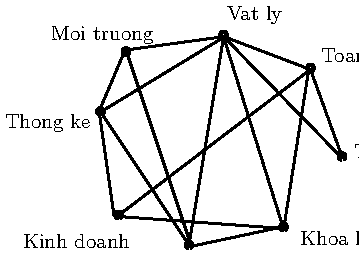
\includegraphics[scale =1]{kithi1}
\caption{}\label{fig:hinh4}
\end{minipage}
\hfill
\begin{minipage}[b]{9cm}
\begin{tabular}{ l  l }
 Tên sinh viên & Môn đã chọn học \\
\hline
 An & Vật lí, Toán, Tiếng Anh \\
Vân& Vật lí, Khoa học trái đất, Kinh tế\\
Lan & Khoa học trái đất, Kinh doanh\\
Hào &Thống kê, Kinh tế\\
Hùng&Toán, Kinh doanh\\
Bảo&Vật lí, Khoa học trái đất\\
Hồng& Kinh doanh, Thống kê\\
Điền &Toán, Khoa học trái đất\\
Cường&Vật lí, Môi trường, Thống kê\\
Quý&Vật lí, Kinh tế, Môi trường.
\end{tabular}
\caption{}\label{fig:hinh00}
\end{minipage}
\end{figure}
Các đợt thi phải bố trí như sau để các sinh viên có thể thi được:

Đợt 1: Vật lí, Kinh doanh

Đợt 2: Toán, Kinh tế

Đợt 3: Tiếng Anh, Khoa học trái đất, Thống kê

Đợt 4: Môi trường.
\end{answer}
\end{question}

\begin{question}%3
Hãy phát biểu định nghĩa và các tính chất của đồ thị Kuratowski. Chứng minh rằng đồ thị  hình ~\ref{fig:hinh5} là không phẳng.
\begin{figure}[!ht]
\begin{minipage}[b]{5cm}
\centering
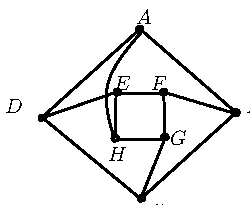
\includegraphics[scale =1]{dothiphang1}
\caption{}\label{fig:hinh5}
\end{minipage}
\hfill
\begin{minipage}[b]{9cm}
\centering
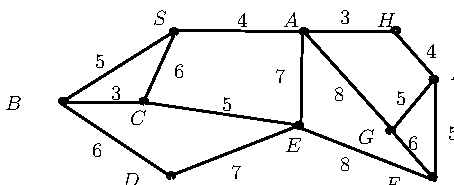
\includegraphics[scale =1]{thuattoan1}
\caption{}\label{fig:hinh7}
\end{minipage}
\end{figure}
\begin{answer}
Định nghĩa: Đồ thị đầy đủ $K_5$ và đồ thị hai phần đầy đủ $K_{3,3}$ được gọi chung là {\it đồ thị Kuratowski}.

Tính chất: Đồ thị Kuratowski là đồ thị không phẳng. (0.5 điểm).

Ta có định lí: Nếu một đồ thị chứa một đồ thị con không phẳng, thì đồ thị đó cũng không phẳng. 

Ta vẽ lại đồ thị hình ~\ref{fig:hinh5} thành đồ thị của hình ~\ref{fig:hinh6}

\begin{figure}[!ht]
\centering
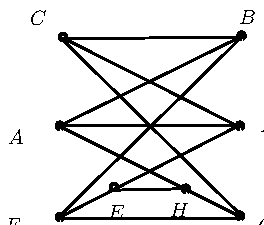
\includegraphics[scale =1]{dothiphang2}
\caption{}\label{fig:hinh6}
\end{figure}

Đồ thị hình ~\ref{fig:hinh6} chứa cấu hình $K_{3,3}$ do đó nó không là đồ thị phẳng.
\end{answer}
\end{question}

\begin{question}%4
\word{{Phương án 1. Trình bày thuật toán Prime. Dùng thuật toán Prime tìm cây bao trùm có trọng số nhỏ nhất trong đồ thị trong hình ~\ref{fig:hinh7}, bắt đầu từ đỉnh $S$.
}{Phương án 2. Trình bày thuật toán Dijsttra. Dùng thuật toán Dijsttra tìm cây bao trùm có trọng số nhỏ nhất trong đồ thị trong hình ~\ref{fig:hinh7}, bắt đầu từ đỉnh $A$.}}
\begin{answer}
Tìm cây bao trùm nhỏ nhất Prim ($MSTPrim$)

\begin{figure}[!ht]
\centering
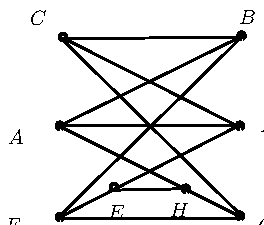
\includegraphics[scale =1]{dothiphang2}
\caption{}\label{fig:hinh8}
\end{figure}

Procedure $MSTPrim$

Đầu vào: Đồ thị liên thông trọng số $\mathcal G$. 

Đầu ra:  Cây bao trùm nhỏ nhất $\mathcal T$.

 1. Chọn đỉnh bất kì $S$ của đồ thị $\mathcal G$;

 2. Khởi tạo  cây Prim  $\mathcal T$ bằng đỉnh  $S$;

 3.  Khởi tạo tập cạnh biên của cây $\mathcal T$ bằng  $\emptyset$;

 4. WHILE {{\it $<$ Cây Prim $\mathcal T$ chưa bao trùm  $\mathcal G>$}}

5.  Cập nhật tập hợp cạnh biên của $\mathcal T$;

6.  Chọn cạnh biên $e$ của cây $\mathcal  T$ có trọng số nhỏ nhất;

7.  Lấy $W$ một điểm cuối của cạnh $e$ mà nằm ngoài $\mathcal T$;

8. Thêm cạnh $e$ (và đỉnh $W$) vào cây $\mathcal  T$;

9. Return (Cây $\mathcal  T$ và nhãn của $C_G(V)$).

10. Kết thúc $MSTPrim$
%}

Các bước tìm kiếm như hình ~\ref{fig:hinh8} :
\end{answer}
\end{question}
\end{shortanswer}


\end{document}




